\documentclass[11pt]{article}
\usepackage[margin=0.9in]{geometry}
\usepackage{amsmath,amssymb,booktabs,graphicx,hyperref,microtype,array,enumitem,caption,placeins,xcolor}
\setlength{\emergencystretch}{2em}\setlength{\parindent}{0pt}\setlength{\parskip}{0.5em}
\captionsetup{font=small,labelfont=bf}
\graphicspath{{figures/}{../../docs/assets/publication/}}
\hypersetup{colorlinks=true,linkcolor=blue!45!black,citecolor=blue!45!black,urlcolor=blue!55!black,pdftitle={Symmetric Factorized Quadratic Adaptation: A Controlled Study of Nonlinear Low-Rank Adapters for GPT-2},pdfauthor={Federico Lolli},pdfsubject={Parameter-efficient fine-tuning and quadratic low-rank adaptation},pdfkeywords={LoRA, PEFT, quadratic adaptation, GPT-2, low-rank adaptation, Transformers, parameter-efficient fine-tuning}}
\newcommand{\sym}{\textsc{Symmetric}}\newcommand{\lora}{\textsc{LoRA}}
\begin{document}
\special{pdf:minorversion 7}
\begin{titlepage}\centering\vspace*{2.2cm}
{\small\sffamily\bfseries RESEARCH PROJECT 01\\[.3em]FEDERICO LOLLI AI RESEARCH\par}\vspace{1.7cm}
{\huge\bfseries Symmetric Factorized Quadratic Adaptation\par}\vspace{.4cm}
{\Large A Controlled Study of Nonlinear Low-Rank Adapters for GPT-2\par}\vspace{2cm}
{\Large Federico Lolli\par}\vspace{.3cm}{\href{mailto:xxlilloxx@gmail.com}{xxlilloxx@gmail.com}\par}
\vfill{\large Independent exploratory research manuscript\par}\vspace{.3cm}{September 2026\par}\vspace{1cm}
\end{titlepage}
\begin{abstract}
Parameter-efficient fine-tuning adapts pretrained models through small modules while leaving the backbone frozen. This study asks whether a low-rank adapter gains useful capacity by replacing the linear \lora{} correction with an explicit quadratic function of projected activations. The proposed \sym{} adapter projects an activation to a low-dimensional space, squares its coordinates element by element, and maps them back; it has the same trainable matrix shapes and parameter count as matched \lora{}. An independent 24-run WikiText-2 confirmation covers ranks 1, 2, 4, and 8, three seeds, and 5,000 optimizer steps. \sym{} obtains lower mean final validation and held-out test loss at every tested rank, with all twelve paired test comparisons favouring it. A six-run AG News classification study provides the counter-result: \lora{} achieves higher mean accuracy and macro-F1. A single-seed scaling ablation and fresh convergence trajectories qualify the rank result. Analytical and empirical studies show that \lora{} has an input-independent Jacobian and zero adapter-only Hessian, whereas \sym{} has an activation-dependent local Jacobian and explicit second-order response. A matched rank-4 benchmark finds nearly identical latency and a 1.25~MiB increase in peak allocated VRAM. The evidence supports quadratic activation-space adaptation as a viable, task-dependent design point rather than a universally superior replacement for linear low-rank adaptation.
\end{abstract}
\tableofcontents\newpage

\section{Introduction}
Full fine-tuning updates every model weight, whereas parameter-efficient fine-tuning (PEFT) freezes most pretrained parameters and learns a small correction. This reduces task-specific state and makes the correction's functional form a meaningful experimental variable. \lora{}~\cite{hu2022lora} is a natural baseline: it is simple, parameter efficient, and interpretable as one constant low-rank weight update. Its adapter branch is nevertheless linear in the incoming activation and cannot itself express second-order feature interactions.

This study evaluates a small change in function class. The incoming activation is projected to $r$ coordinates, those coordinates are squared element by element, and the result is projected back. This preserves the trainable shapes of \lora{} while making the correction quadratic and activation dependent. A controlled comparison is necessary because rank, parameter count, placement, scaling, training duration, seed, and task can all alter the observed ordering.

\subsection{Research question}
Can a low-rank adapter gain useful expressive capacity by replacing the purely linear \lora{} correction with an explicit quadratic function of projected activations, while retaining a comparable parameter budget and practical computational cost? The question matters because adapters of identical size can implement different local transformations.

\subsection{Contributions}
This work provides (i) a precise symmetric factorized quadratic activation-space adapter; (ii) controlled comparisons with \lora{} under matched budgets; (iii) rank, scaling, convergence, placement, and downstream analyses; (iv) local-Jacobian, effective-rank, and adapter-Hessian analyses; (v) a matched cost benchmark; and (vi) conservative positioning relative to verified related methods. These are empirical and analytical contributions, not a claim of universal novelty or superiority. Sections~2--4 introduce the context, method, and protocols; Sections~5--8 present results, mechanism analysis, and cost; Sections~9--11 discuss scope and conclusions.

\section{Related work and positioning}
Table~\ref{tab:related} compares mechanisms rather than incompatible benchmark scores. Only \lora{} is reproduced as a direct baseline.
\begin{table}[ht]\centering\small
\caption{Mathematical and architectural positioning. External methods were not experimentally reproduced.}\label{tab:related}
\begin{tabular}{p{.13\linewidth}p{.38\linewidth}p{.39\linewidth}}\toprule
Method&Core mechanism&Relation to this study\\\midrule
\lora{}&Low-rank linear correction&Direct baseline\\
DoRA&Weight magnitude/direction decomposition&Different weight parameterization\\
MoRA&Square trainable matrix with fixed transforms&Weight-space high-rank strategy\\
HiRA&Hadamard-product high-rank update&Weight-space higher-rank adaptation\\
LoRAN&Nonlinear low-rank weight update&Nonlinear weight-space method\\
PERA&Polynomial expansion of low-rank factors&Higher-order parameter/factor-space method\\
QuadraNet V2&Factorized quadratic neural transformation&Related quadratic-form precedent\\
This study&Squared projected activation&Activation-dependent quadratic correction\\\bottomrule
\end{tabular}\end{table}
\lora{} learns a linear update~\cite{hu2022lora}. DoRA separates weight magnitude and direction~\cite{liu2024dora}; MoRA uses a square matrix and fixed transforms~\cite{jiang2024mora}; HiRA forms a Hadamard-product update~\cite{huang2025hira}; and LoRAN transforms a low-rank weight update nonlinearly~\cite{li2024loran}. These operate in weight or parameter space rather than by squaring the current activation.

\subsection{PERA} PERA expands low-rank factors polynomially before composition~\cite{zhang2026pera}. This study follows $x\to xU\to(xU)\odot(xU)\to P$. Both investigate higher-order structure, but the operation acts on different objects. PERA is not an experimental baseline here.

\subsection{QuadraNet V2} QuadraNet V2 is a verified precedent for factorized quadratic transformations~\cite{xu2026quadranet}. For one output, the present adapter is $xQ_jx^T$. Across a multi-output layer, all $Q_j$ share directions in $U$ and differ through coefficients in $P$; single-output similarity does not establish full architectural equivalence.

\subsection{Position of the proposed method} The defining feature is the element-wise square after the activation projection and before the output projection. This yields an input-dependent local transformation at matched \lora{} size. Figure~\ref{fig:related} later summarizes where higher-order operations enter the compared methods.

\section{Method}
\subsection{Frozen projection and parallel correction}
For row activation $x\in\mathbb{R}^{1\times d}$, frozen $W\in\mathbb{R}^{d\times d_{out}}$, and frozen bias $b$,
\begin{equation}y_{base}=xW+b.\label{eq:base}\end{equation}
The adapter is a parallel trainable branch. Matched \lora{} and \sym{} corrections are
\begin{align}
\Delta y_{\mathrm{LoRA}}&=\frac{\alpha}{r}(xA)B,\label{eq:lora}\\
\Delta y_{\mathrm{Sym}}&=\frac{\alpha}{r}\bigl((xU)\odot(xU)\bigr)P,\label{eq:sym}
\end{align}
where $A,U\in\mathbb{R}^{d\times r}$ and $B,P\in\mathbb{R}^{r\times d_{out}}$. Both contain $r(d+d_{out})$ parameters, or $2dr$ for square GPT-2 \texttt{c\_proj}. \lora{} applies two linear projections; \sym{} forms $z=xU$, computes $z\odot z$, then applies $P$.
\begin{figure}[ht]\centering\includegraphics[width=\textwidth]{adapter_architecture_comparison_for_paper.png}
\caption{Architecture of matched \lora{} and \sym{} adapters. Both add a low-rank trainable branch beside a frozen projection. \lora{} is linear; \sym{} inserts an element-wise square before the output projection.}\label{fig:architecture}\end{figure}

\subsection{Quadratic structure}
For output $j$,
\begin{align}\Delta y_j&=\frac{\alpha}{r}\sum_kP_{kj}(xu_k)^2=xQ_jx^T,\label{eq:coord}\\Q_j&=\frac{\alpha}{r}U\operatorname{diag}(P_{:,j})U^T.\label{eq:qj}\end{align}
$Q_j$ is symmetric and $\operatorname{rank}(Q_j)\le r$. Directions in $U$ are shared across outputs; signed coefficients in $P$ mean $Q_j$ need not be positive semidefinite. The identity $(ax_1+bx_2)^2=a^2x_1^2+2abx_1x_2+b^2x_2^2$ shows that squared projections create cross terms. Output factors are zero initialized. The main study uses $\alpha=4$, giving $\alpha/r=4,2,1,0.5$ at ranks 1,2,4,8 and motivating Section~\ref{sec:scaling}.

\subsection{GPT-2 insertion point}
The controlled adapter receives the concatenated attention output entering zero-based block 0 \texttt{attn.c\_proj}. Frozen projection and adapter outputs are summed before attention residual dropout and residual addition (Figure~\ref{fig:placement}).
\begin{figure}[ht]\centering\includegraphics[width=.94\textwidth]{gpt2-attn-adapter-path.pdf}
\caption{Controlled GPT-2 placement. The trainable adapter and frozen block-0 \texttt{attn.c\_proj} share an input; their outputs are summed before residual dropout and the attention residual addition. Block numbering is zero based.}\label{fig:placement}\end{figure}

\FloatBarrier\section{Experimental design}
Historical studies motivated controlled questions but are not pooled with them. Table~\ref{tab:campaigns} records each campaign's role.
\begin{table}[ht]\centering\small
\caption{Completed experimental campaigns.}\label{tab:campaigns}
\begin{tabular}{p{.2\linewidth}p{.49\linewidth}p{.21\linewidth}}\toprule
Campaign&Design&Role\\\midrule
Adapter families&Linear, quadratic, interaction, symmetric, mixed variants&Exploration\\
Depth/placement&Attention/MLP screens and 12-block scan&Placement\\
Fixed-budget multilayer&6,144/12,288 parameters across layers&Depth/local rank\\
AG News&Two methods, three seeds, 500 steps&Classification\\
Rank screening&Two methods, four ranks, three seeds, 1,000 steps&Screening\\
Rank confirmation&24 fresh runs, 5,000 steps&Central LM evidence\\
Scaling ablation&$\alpha=4$ versus $\alpha/r=1$, seed 42&Scale check\\
Mechanism/cost&Stored checkpoints; matched rank-4 benchmark&Structure/cost\\\bottomrule
\end{tabular}\end{table}

\subsection{Historical exploration} Early adapter-family studies, 500/1,000/2,000-step durations, attention and MLP screens, a 12-block attention scan, and fixed-budget multilayer designs established trainability and motivated later controls. Their nonuniform protocols remain separate; Appendix~\ref{app:history} summarizes verified values.

\subsection{Controlled WikiText-2 protocol} GPT-2 Small is frozen. WikiText-2 is packed into consecutive 128-token blocks for causal cross-entropy. Runs use block 0 \texttt{attn.c\_proj}, batch 1, accumulation 4, AdamW at $3\times10^{-4}$, clipping 1.0, no scheduler, $\alpha=4$, ranks 1/2/4/8, seeds 42/123/456, and 5,000 steps. The 1,000-step screen is independent. Best recorded validation, exact final validation, and final-checkpoint held-out test are distinct; test data select nothing.

\subsection{Controlled AG News protocol} The same frozen backbone and placement are used with a classification head, 4,096 training examples, a fixed 1,000-example stratified validation subset, the original test split, rank 4, three seeds, and 500 steps. Each method has 9,216 trainable parameters including the head.

\subsection{Scaling ablation} A seed-42, 1,000-step ablation compares fixed $\alpha=4$ with constant $\alpha/r=1$ ($\alpha=r$). It is exploratory and separate from the main confirmation.

\subsection{Mechanism and cost protocols} Final checkpoints are reused for spectra, output covariance, local Jacobians, and adapter-only Hessians on fixed held-out activations. Analytical derivatives are checked against double-precision autograd. The cost benchmark uses rank 4, batch 1, sequence length 128, 10 warm-up and 30 measured iterations. No full-block Hessian was completed.

\FloatBarrier\section{Controlled results}
\subsection{WikiText-2 confirmation}
Table~\ref{tab:rank} reports final-checkpoint means and sample SD. Lower is better.
\begin{table}[ht]\centering
\caption{Final WikiText-2 loss over three seeds.}\label{tab:rank}
\begin{tabular}{rcccc}\toprule Rank&\lora{} val&\sym{} val&\lora{} test&\sym{} test\\\midrule
1&$3.5734\pm0.0051$&$3.5314\pm0.0207$&$3.9256\pm0.0009$&$3.9131\pm0.0042$\\
2&$3.4773\pm0.0057$&$3.4340\pm0.0249$&$3.8492\pm0.0025$&$3.8305\pm0.0144$\\
4&$3.3483\pm0.0093$&$3.3101\pm0.0011$&$3.7656\pm0.0054$&$3.7429\pm0.0024$\\
8&$3.3054\pm0.0117$&$3.2446\pm0.0096$&$3.7319\pm0.0035$&$3.6938\pm0.0044$\\\bottomrule\end{tabular}\end{table}
Paired test differences (\sym{} minus \lora{}) are $-0.0125\pm0.0051$, $-0.0187\pm0.0119$, $-0.0227\pm0.0035$, and $-0.0381\pm0.0072$ at ranks 1,2,4,8; all 12 pairs favour \sym{}. Figure~\ref{fig:rank} shows individual seeds and SD. This result is specific to the tested task, placement, schedule, and scale.
\begin{figure}[ht]\centering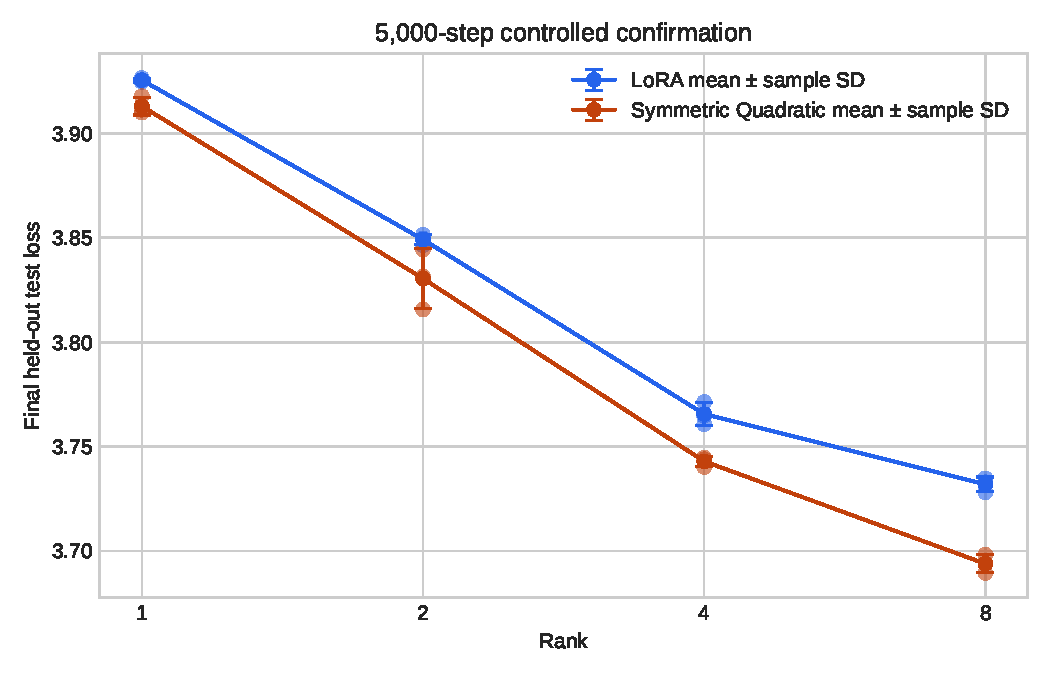
\includegraphics[width=.82\textwidth]{rank_5000_final_test_loss.pdf}
\caption{Held-out WikiText-2 test loss after 5,000 steps at ranks 1,2,4,8. Lower is better. Points are seeds; markers/error bars are mean/sample SD. \sym{} is lower on average at every rank in this protocol.}\label{fig:rank}\end{figure}

\subsection{AG News}
\begin{table}[ht]\centering\caption{AG News held-out results, mean $\pm$ sample SD.}\label{tab:ag}
\begin{tabular}{lccc}\toprule Method&Accuracy&Macro-F1&Test loss\\\midrule
\lora{}&$0.8201\pm0.0051$&$0.8156\pm0.0050$&$0.5445\pm0.0542$\\
\sym{}&$0.8021\pm0.0240$&$0.7929\pm0.0315$&$0.6847\pm0.1919$\\\bottomrule\end{tabular}\end{table}
\lora{} is better on average for all three measures. Figure~\ref{fig:ag} exposes the larger \sym{} seed variability, demonstrating that the WikiText-2 ordering does not transfer automatically.
\begin{figure}[ht]\centering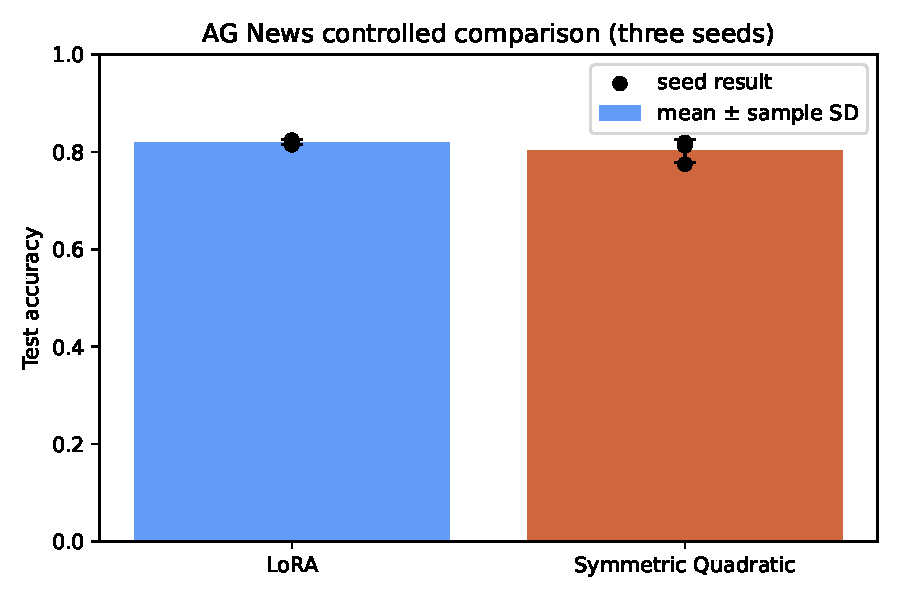
\includegraphics[width=.72\textwidth]{downstream_accuracy_comparison.pdf}
\caption{AG News held-out accuracy. Bars/error bars are mean/sample SD; black points show all seeds. \lora{} is higher on average.}\label{fig:ag}\end{figure}

\FloatBarrier\section{Scaling and convergence}\label{sec:scaling}
\subsection{Constant-scale ablation}
\begin{table}[ht]\centering\small\caption{Seed-42 validation loss after 1,000 steps; $\Delta=\sym{}-\lora{}$.}\label{tab:scale}
\begin{tabular}{rccc@{\hspace{1em}}ccc}\toprule&\multicolumn{3}{c}{$\alpha=4$}&\multicolumn{3}{c}{$\alpha/r=1$}\\Rank&\lora{}&\sym{}&$\Delta$&\lora{}&\sym{}&$\Delta$\\\midrule
1&3.6171&3.6614&+.0443&3.6301&3.6711&+.0410\\2&3.5861&3.5561&-.0300&3.5984&3.5693&-.0292\\4&3.5530&3.4780&-.0750&3.5530&3.4780&-.0750\\8&3.5492&3.4315&-.1177&3.5056&3.4081&-.0975\\\bottomrule\end{tabular}\end{table}
The sign pattern persists for seed 42 while magnitude changes (Figure~\ref{fig:scale}); one seed prevents broader inference.
\begin{figure}[ht]\centering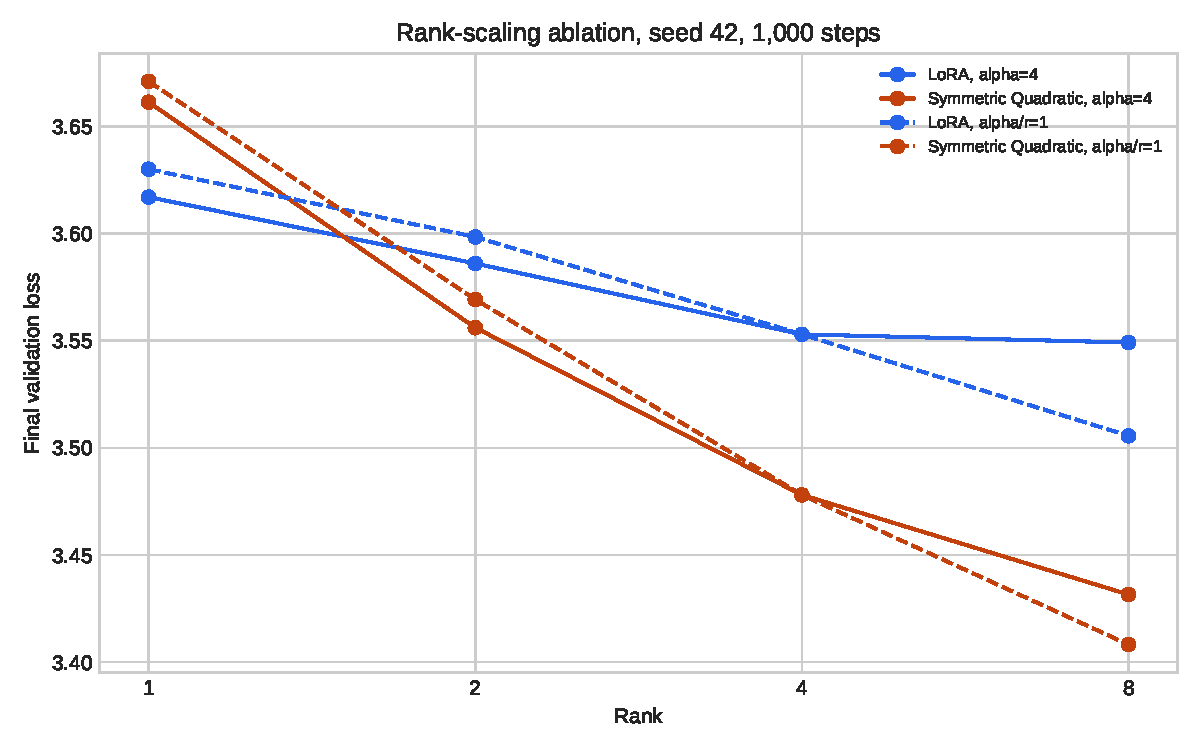
\includegraphics[width=.8\textwidth]{rank_scaling_ablation_loss.pdf}
\caption{Single-seed scaling ablation. Fixed $\alpha$ changes effective scale with rank; the comparison fixes $\alpha/r=1$.}\label{fig:scale}\end{figure}

\subsection{Fresh confirmation trajectories}
\begin{table}[ht]\centering\caption{Mean paired validation difference $\sym{}-\lora{}$.}\label{tab:conv}
\begin{tabular}{rccccc}\toprule Rank&1,000&2,000&3,000&4,000&5,000\\\midrule
1&+.0280&+.0096&-.0043&-.0265&-.0419\\2&-.0367&-.0432&-.0319&-.0311&-.0434\\4&-.0707&-.0631&-.0803&-.0635&-.0382\\8&-.1247&-.1156&-.0947&-.0781&-.0608\\\bottomrule\end{tabular}\end{table}
Negative favours \sym{}. Rank 1 crosses between 2,000 and 3,000 recorded steps; ranks 2--8 favour \sym{} at every listed point. The independent screen is not joined to these curves. Figure~\ref{fig:conv} shows rank 1 and SD; no asymptotic claim is made.
\begin{figure}[ht]\centering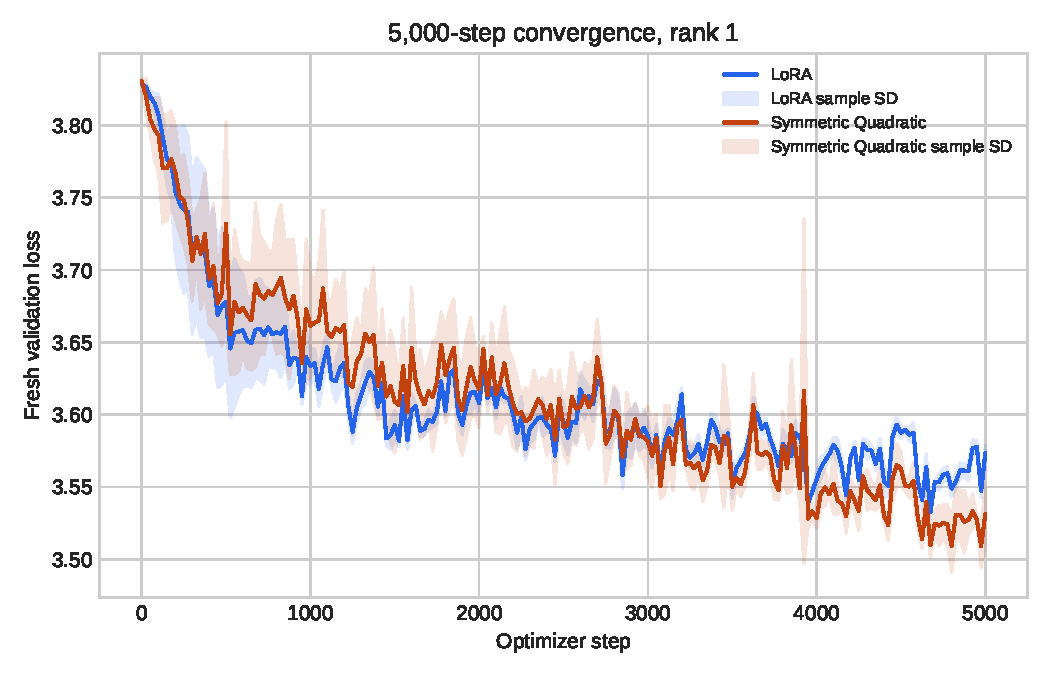
\includegraphics[width=.82\textwidth]{convergence_rank1.pdf}
\caption{Fresh rank-1 validation trajectories in the 5,000-step confirmation. Curves are means; bands are sample SD.}\label{fig:conv}\end{figure}

\FloatBarrier\section{Mechanism analysis}
These analyses characterize structure but do not establish why performance differs.
\subsection{Local Jacobians}
\begin{align}J_{\mathrm{LoRA}}&=\frac{\alpha}{r}AB,\label{eq:jl}\\J_{\mathrm{Sym}}(x)&=2\frac{\alpha}{r}U\operatorname{diag}(xU)P.\label{eq:js}\end{align}
\lora{} is input independent and represents one fixed local update. \sym{} changes with $x$ and cannot generally be reduced to one constant $\Delta W$. Double-precision tests match these expressions to autograd.

\subsection{Effective rank}
Entropy effective rank is $\exp(-\sum_i p_i\log p_i)$ for normalized singular values $p_i$. Table~\ref{tab:erank} reports distinct objects.
\begin{table}[ht]\centering\caption{Mean entropy effective ranks.}\label{tab:erank}
\begin{tabular}{rccccc}\toprule Rank&\lora{} update&\sym{} Jacobian&$U$&$P$&Output cov.\\\midrule
1&1.00&1.00&1.00&1.00&1.00\\2&1.92&1.67&2.00&1.98&1.92\\4&3.76&3.09&3.99&3.89&3.00\\8&6.57&5.59&7.96&7.28&3.59\\\bottomrule\end{tabular}\end{table}
The \sym{} local-Jacobian rank is not a fixed weight-update rank directly equivalent to \lora{} (Figure~\ref{fig:jac}).
\begin{figure}[ht]\centering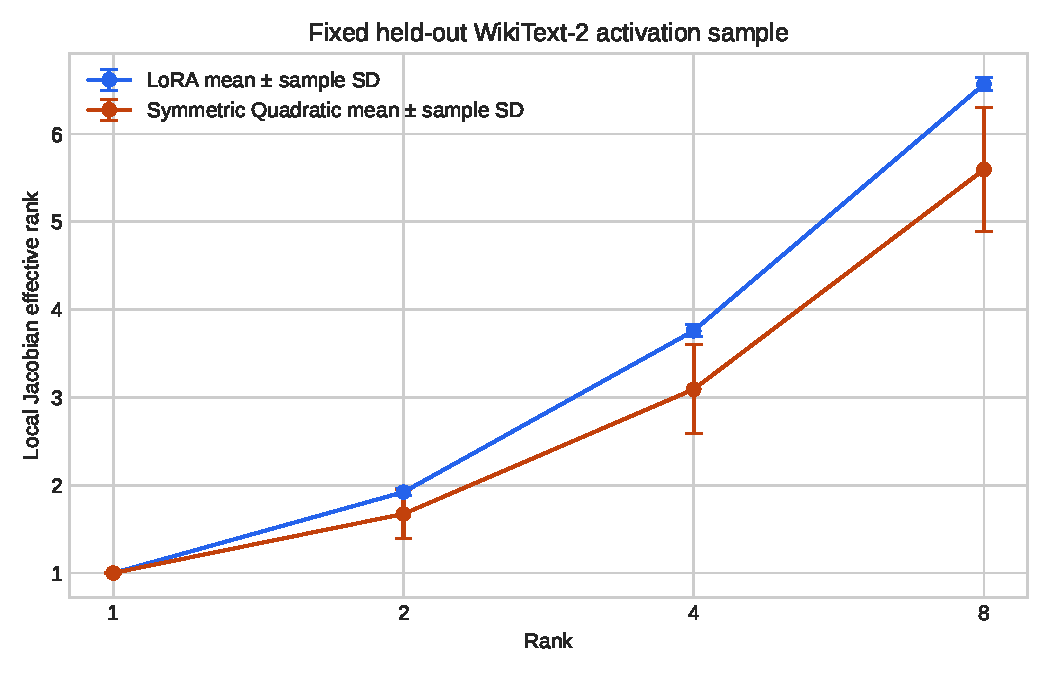
\includegraphics[width=.8\textwidth]{jacobian_effective_rank.pdf}
\caption{Effective rank of the \lora{} update and \sym{} local Jacobian. These measure related local complexity but are not identical weight-space objects.}\label{fig:jac}\end{figure}

\subsection{Second-order structure}
For fixed linear output reduction $c$,
\begin{equation}H=2\frac{\alpha}{r}U\operatorname{diag}(Pc)U^T.\label{eq:hess}\end{equation}
\lora{} has zero adapter-only Hessian; \sym{} is nonzero. Mean \sym{} Frobenius norms are 155.15, 92.13, 52.68, 17.61 at ranks 1,2,4,8. The decrease combines learned factors and scale and is not evidence of weaker useful interactions. For fixed $c$, the Hessian is input independent, so repeated tokens are not independent observations. Autograd verifies Equation~\ref{eq:hess}; a full-block Hessian was not evaluated.
\begin{figure}[ht]\centering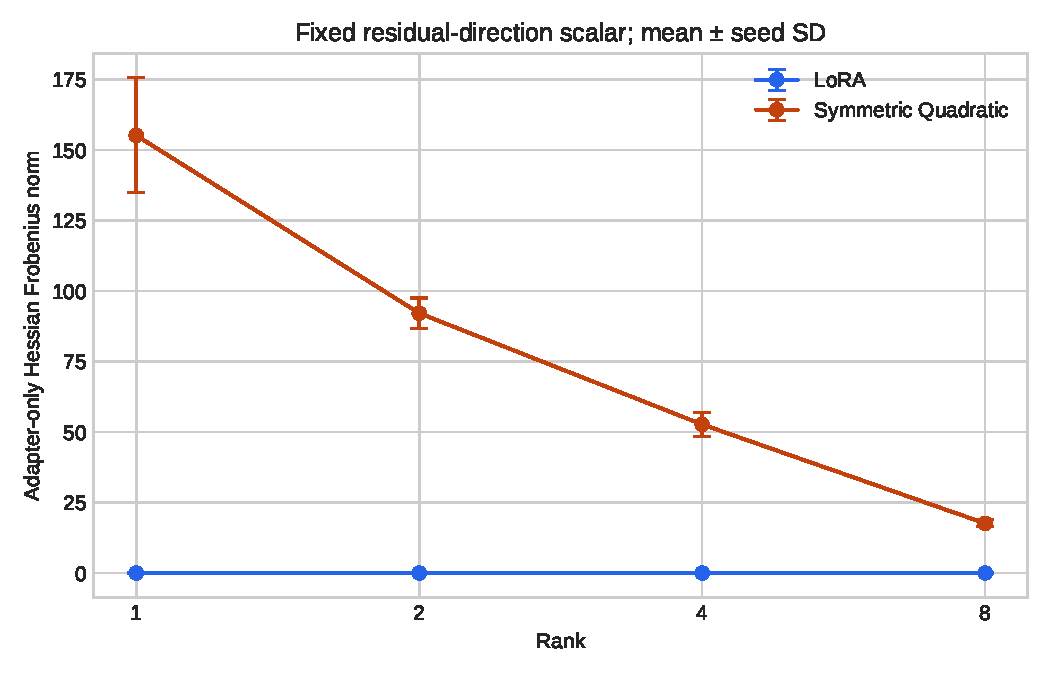
\includegraphics[width=.8\textwidth]{adapter_interaction_hessian.pdf}
\caption{Adapter-only second-order response. \lora{} is exactly zero; \sym{} has an explicit nonzero response. This does not prove a causal performance mechanism.}\label{fig:hess}\end{figure}

\FloatBarrier\section{Computational cost}
Both rank-4 adapters have 6,144 parameters. Table~\ref{tab:cost} shows nearly identical measured cost.
\begin{table}[ht]\centering\caption{Matched rank-4 benchmark: batch 1, length 128, 10 warm-up and 30 measured iterations.}\label{tab:cost}
\begin{tabular}{lrrrr}\toprule Method&Forward (ms)&Backward (ms)&VRAM (MiB)&Tokens/s\\\midrule
\lora{}&$12.157\pm0.243$&$14.805\pm0.236$&429.05&10,529\\\sym{}&$12.184\pm0.236$&$14.766\pm0.188$&430.31&10,505\\\bottomrule\end{tabular}\end{table}
Relative differences are approximately $+0.22\%$ forward latency, $-0.27\%$ backward latency, $+1.25$~MiB VRAM, and $-0.22\%$ throughput. The result applies only to this implementation and hardware configuration.

\section{Discussion}
The controlled WikiText-2 result is positive and configuration specific: \sym{} is lower at every rank and in every paired held-out comparison. AG News favours \lora{} on average, showing task dependence. Rank and optimization duration matter: rank 1 changes ordering during training, while higher-rank gaps narrow over the recorded interval. Constant scale alters magnitude but does not change the tested seed's qualitative pattern; the design does not fully isolate rank, scale, and parameter count.

The derivative study guarantees a structural distinction and measures learned spectra, but does not prove that second-order response causes lower language-model loss. The cost study shows that this structure can be implemented at almost the same measured practical cost. Figure~\ref{fig:related} summarizes the architectural context without implying equivalence.
\begin{figure}[ht]\centering\includegraphics[width=\textwidth]{adapter-family-comparison.pdf}
\caption{Architectural comparison of \lora{}, \sym{}, PERA, QuadraNet V2, and a nonlinear bottleneck adapter. The location of a higher-order operation differs; visual similarity does not imply mathematical equivalence.}\label{fig:related}\end{figure}

\section{Limitations}
Evidence is limited to GPT-2 Small, two datasets, restricted placements, three central seeds, one scaling-ablation seed, and no exhaustive hyperparameter sweep. Related methods except \lora{} were not reproduced. There is no full-block Hessian, and cost was measured for one rank, device, batch size, and sequence length. The literature review does not establish universal novelty over every quadratic architecture.

\section{Conclusion}
\sym{} is a viable quadratic activation-space adapter. Under controlled 5,000-step WikiText-2 conditions, it achieves lower mean final validation and held-out test loss than matched \lora{} at ranks 1,2,4,8. AG News favours \lora{} on average, so the evidence is task dependent. Rank, scaling, and duration qualify the result. Jacobian and Hessian analyses establish functional differences, while the matched benchmark finds small overhead. Adapter functional form therefore matters alongside parameter count, but broader generalization requires additional models, tasks, placements, and replications.

\appendix
\section{Per-seed results and provenance}
Per-seed WikiText-2 values are available in \path{results/tables/rank-confirmation-5000/rank_5000_per_seed.csv}; AG News runs are in \path{results/tables/downstream-ag-news/downstream_controlled_results.csv}. Aggregate tables in this paper are reconstructed from those files without cherry-picking. Figure provenance is recorded in \path{results/manifests/FIGURE_MANIFEST.md}.

\section{Historical evidence}\label{app:history}
Historical best-recorded validation summaries include, at 500 steps: \lora{} 3.5732, element-wise quadratic 3.6351, signed quadratic 3.6257, interaction 3.5581, \sym{} 3.5526, and Linear+Quadratic 3.5302. At one rank-4 insertion point, 1,000-step summaries were 3.5491, 3.4770, 3.4928 for \lora{}, \sym{}, Linear+Quadratic; at 2,000 steps they were 3.4598, 3.3784, 3.4360. These exploratory results motivated controls but are not merged with confirmation trajectories.

\section{Reproducibility notes}
Canonical tables are under \path{results/tables/}; commands and recorded software/hardware details are in \path{research/reproducibility/REPRODUCIBILITY.md}. Analytical Jacobian, Hessian, spectral, aggregation, and public-data tests are part of the repository suite. Raw private checkpoints are not embedded in the public manuscript.

\begin{thebibliography}{9}
\bibitem{hu2022lora} E. J. Hu et al. \emph{LoRA: Low-Rank Adaptation of Large Language Models}. ICLR, 2022.
\bibitem{liu2024dora} S.-Y. Liu et al. \emph{DoRA: Weight-Decomposed Low-Rank Adaptation}. ICML, 2024.
\bibitem{jiang2024mora} T. Jiang et al. \emph{MoRA: High-Rank Updating for Parameter-Efficient Fine-Tuning}. arXiv:2405.12130, 2024.
\bibitem{huang2025hira} Q. Huang et al. \emph{HiRA: Parameter-Efficient Hadamard High-Rank Adaptation for Large Language Models}. ICLR, 2025.
\bibitem{li2024loran} Y. Li, L. Song, and H. Hou. \emph{LoRAN: Improved Low-Rank Adaptation by a Non-Linear Transformation}. Findings of EMNLP, 2024.
\bibitem{zhang2026pera} W. Zhang et al. \emph{Polynomial Expansion Rank Adaptation: Enhancing Low-Rank Fine-Tuning with High-Order Interactions}. Findings of ACL, 2026. DOI: \href{https://doi.org/10.18653/v1/2026.findings-acl.650}{10.18653/v1/2026.findings-acl.650}.
\bibitem{xu2026quadranet} C. Xu et al. \emph{QuadraNet V2: Efficient and Sustainable Training of High-Order Neural Networks with Quadratic Adaptation}. WACV, 2026.
\end{thebibliography}
\end{document}
